Die Ströme und Spannungen konnten teilweise nur indirekt gemessen werden und
mussten daher aus mehreren Messungen berechnet werden.

\subsubsection{ES\_IGK1}
Der Kollektorstrom $I_C$ der Schaltung wurde durch die Messung der Spannung über dem
Widerstand $R_3$ ($V_2 - U_C$)und entsprechender Division durch dessen Widerstandswert
ermittelt.
\[I_C  = \frac{V_2 - U_c}{R_3} = \frac{12.01 \, \si{\volt} - 6.38 \,
    \si{\volt}}{1.3 \, \si{\kilo\ohm}} = 4.33 \, \si{\milli\ampere}\]

Die Kollektorspannung konnte dann über Messung des Emitterpotentials $U_E$ gegen Masse
und Differenzbildung mit dem vorher bestimmten Wert $U_c$ bestimmt werden.
\[U_{CE} = U_C - U_E = 6.38 \, \si{\volt} - 0.436 \, \si{\volt} = 5.944 \, \si{\volt}\]

Der Basisstrom ist die Differenz aus dem Strom durch $R_1$ und dem Strom durch
$R_2$.
\[I_B = \frac{V_2 - U_B}{R_1}-\frac{U_B}{R_2} = \frac{12 \, \si{\volt} - 1.149
    \, \si{\volt}}{43 \, \si{\kilo\ohm}} - \frac{1.149 \, \si{\volt}}{5.1 \,
    \si{\kilo\ohm}} = 27.58 \, \si{\micro\ampere}\]

Die statische Stromverstärkung ist damit
\[B = \frac{I_C}{I_B} = \frac{4.33 \, \si{\milli\ampere}}{27.58 \,
    \si{micro\ampere}} = 157\]

Aus dem Datenblatt des 2N3904 Bipolartransistors lässt sich bei einem
Kollektorstrom vom etwa $I_C = 4 \, \si{\milli\ampere}$ und einer
Kollektor-Emitter-Spannung von $U_{CE} = 10 \, \si{\volt}$ ein
Stromverstärkungsfaktor von $B = 150$ ablesen. (Datenblatt onsemi Abb. 11).

\begin{figure}[H]
  \begin{center}
    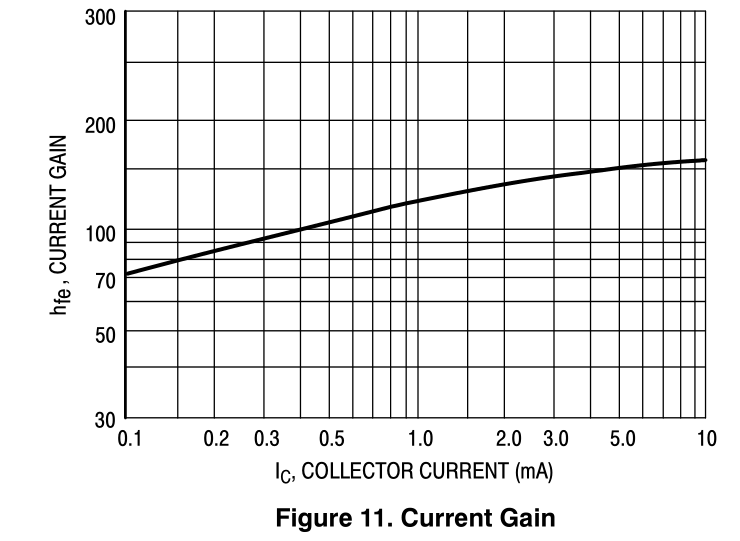
\includegraphics[width=0.618\textwidth]{2_2/ds1}
  \end{center}
  \caption{Quelle: http://onsemi.com}
\end{figure}

\subsubsection{ES\_IUGK1}
Die Arbeitspunktwerte der zweiten und dritten Schaltung wurden entsprechend 2.2.1 bestimmt.

\begin{table}[H]
\begin{center}
\begin{tabular}{c | c}
  $U_C$ & $6.06 \, \si{\volt}$\\
  \hline
  $U_E$ & $0.53 \, \si{\volt}$\\
  \hline
  $U_B$ & $1.23 \, \si{\volt}$\\
\end{tabular}
\end{center}
\caption{Zwischenwerte der Schaltung ES\_IUGK1}
\end{table}

\begin{table}[H]
\begin{center}
\begin{tabular}{c | c}
  $I_C$ & $5.23 \, \si{\milli\ampere}$\\
  \hline
  $U_{CE}$ & $5.53 \, \si{\volt}$\\
  \hline
  $I_{B}$ & $24.15 \, \si{\micro\ampere}$\\
  \hline
  $B$ & $216 $\\
\end{tabular}
\caption{Arbeitspunktwerte der Schaltung ES\_IUGK1}
\end{center}
\end{table}

\subsubsection{KS\_BOS1}

\begin{table}[H]
\begin{center}
\begin{tabular}{c | c}
  $U_C$ & $12.01 \, \si{\volt}$\\
  \hline
  $U_E$ & $4.37 \, \si{\volt}$\\
  \hline
  $U_B$ & $5 \, \si{\volt}$\\
  \hline
  $U_{R1}$ & $6.9 \, \si{\volt}$\\
  \hline
  $U_{R3}$ & $0.63 \, \si{\volt}$\\
\end{tabular}
\end{center}
\caption{Zwischenwerte der Schaltung KS\_BOS1}
\end{table}

\begin{table}[H]
\begin{center}
\begin{tabular}{c | c}
  $I_C$ & $ 1.45 \, \si{\milli\ampere}$\\
  \hline
  $U_{CE}$ & $ 7.91 \, \si{\volt}$\\
  \hline
  $I_{B}$ & $ 4.26 \, \si{\micro\ampere}$\\
  \hline
  $B$ & $340.38$\\
\end{tabular}
\caption{Arbeitspunktwerte der Schaltung KS\_BOS1}
\end{center}
\end{table}

